\documentclass{article}
\usepackage{amsmath}
\usepackage{amssymb}
\usepackage{tikz}
\usetikzlibrary{shapes,decorations,arrows,calc,arrows.meta,fit,positioning}
\tikzset{
    -Latex,auto,node distance =1 cm and 1 cm,semithick,
    state/.style ={ellipse, draw, minimum width = 0.7 cm},
    point/.style = {circle, draw, inner sep=0.04cm,fill,node contents={}},
    bidirected/.style={Latex-Latex,dashed},
    el/.style = {inner sep=2pt, align=left, sloped},
    pdp/.style = {pdpcolor, dash pattern = on 2pt off 4pt, dash phase=3pt, line width=0.8pt},
    % direct effect
    tdp/.style = {tdpcolor, dash pattern = on 2pt off 4pt, line width=0.8pt},
    % total effect
    itdp/.style = {tdpcolor, dash pattern = on 2pt off 1pt, line width=0.8pt},
    % indirect part of total effect
    ecmtdp/.style = {tdpcolor}
    % ECM part of total effect
}

\begin{document}

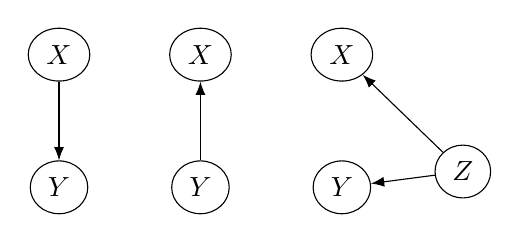
\begin{tikzpicture}
    \node[state] (x) at (0,0) {$X$};
    \node[state] (y) [below = of x] {$Y$};
    \path (x) edge (y);
    \node[state] (x2) [right = of x] {$X$};
    \node[state] (y2) [below = of x2] {$Y$};
    \path (y2) edge (x2);
    \node[state] (x3) [right = of x2] {$X$};
    \node[state] (z) [below right = of x3] {$Z$};
    \node[state] (y3) [below = of x3] {$Y$};
    \path (z) edge (x3);
    \path (z) edge (y3);
\end{tikzpicture}

\end{document}